\chapter{Revisão Bibliográfica} \label{cap2}
\section{Fundamentação Teórica}
\subsection{Redes Neurais}
Redes neurais são modelos computacionais inspirados no sistema nervoso humano. Suas estruturas são subdivididas em camadas e unidades de processamento. As camadas representam a ordem nas quais os neurônios processam as informações. Os neurônios são as unidades de processamento, onde similarmente ao sistema nervoso, recebem um estimulo, processam e transmitem o estimulo aos demais neurônios da rede neural. A estrutura de um neurônio pode ser visto na figura a seguir:
\begin{figure}[h]
	\centering
    \label{fig1}
    \vspace{3ex}%
	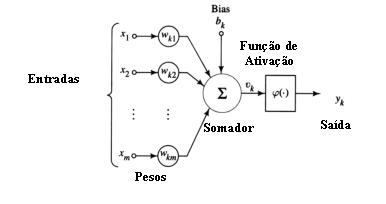
\includegraphics[scale=0.7]{pasta1_figuras/neuronio_artificial.jpg}
    \caption{Neurônio Artificial}
\end{figure}

\subsection{Verificação}
Verificacao aqui
\subsection{GPU}
% Fim Capítulo